\documentclass[10pt,notheorems]{beamer}
\usepackage[utf8]{inputenc}
\usepackage[T1]{fontenc}
\usepackage[french]{babel}
\usepackage{mathtools, amssymb, amsthm}
\usepackage{hyperref}
\usepackage{graphicx}
\usepackage{xcolor}
\usepackage{mathrsfs}
\usepackage{wrapfig}
\usepackage{stmaryrd}
\usepackage{multimedia}
\usetheme{Warsaw}
\setbeamertemplate{theorems}[numbered]

\theoremstyle{plain}
\newtheorem{theorem}{Théorème}[section]

\theoremstyle{definition}
\newtheorem{definition}{Définition}[section]

\theoremstyle{plain}
\newtheorem{prop}{Proposition}

\theoremstyle{plain}
\newtheorem{lemma}{Lemme}

\theoremstyle{plain}
\newtheorem{corollary}{Corollaire}

\theoremstyle{remark}
\newtheorem{remark}{Remarque}


\title{Rubik's cube et la théorie des groupes}
\author{Anastasiia \bsc{Chernetcova}, supervisé par Yves \bsc{Aubry}}
\date{Mars 2022}
\titlegraphic{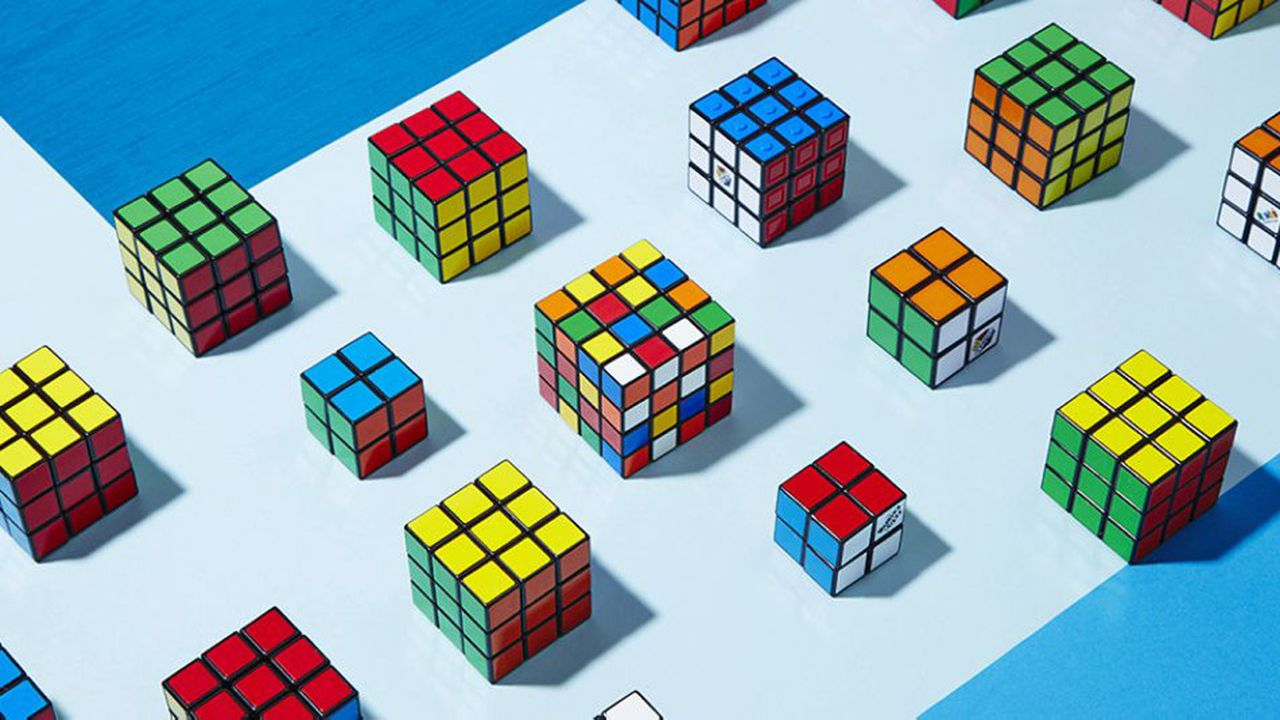
\includegraphics[scale=0.15]{figures/image-titre.jpg}}

\begin{document}

\begin{frame}
\titlepage
\end{frame}

\begin{frame}
  \frametitle{Introduction}
  \begin{enumerate}
    \item Le cube se compose de $3 ^3$ petits cubes ;
    \item 7 sont fixes :
    \begin{enumerate}
      \item le cube central ;
      \item le cube au centre des tranches (3).
    \end{enumerate}
    et 20 mobiles :
    \begin{enumerate}
      \item Les coins, au nombre de 8 (1) ;
      \item Les arêtes, au nombre de 12 (2).
    \end{enumerate}
  \end{enumerate}

  \begin{figure}
    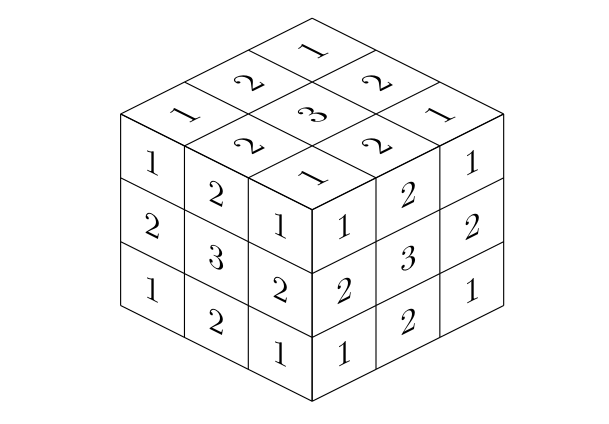
\includegraphics[scale=0.3]{figures/cube_parties_fixes_mobiles.png}
    \caption{Les parties fixes et mobiles du cube}
    \label{cube_parties_fixes_mobiles}
  \end{figure}
\end{frame}

\begin{frame}
  \frametitle{Introduction}
  But du jeu = résoudre le Rubik's cube, ie le ramener dans son état d'origine.

  \begin{figure}
    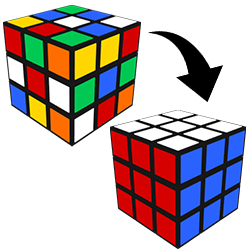
\includegraphics[scale=0.5]{figures/non-resolu.png}
    \caption{Résoudre le Rubik's cube}
    \label{}
  \end{figure}
\end{frame}
%--- Next Frame ---%

\begin{frame}
  \frametitle{Notations et vocabulaire}
  \begin{itemize}
    \item Tranche du Rubik's cube = partie tournante composée de 9 pièces ;
    \item On notera les faces $ U, F, L, R, B, D$.
    \item $U, F, L, R, B, D$ seront aussi les rotations dans le sens des aiguilles d'une montre des mêmes faces. On notera $R ^{-1} $ la rotation dans le sens contraire des aiguilles d'une montre.
  \end{itemize}
\end{frame}
%--- Next Frame ---%

\begin{frame}
  \frametitle{Groupe du Rubik's cube}
  On notera les coins comme indiqué dans la figure \ref{num_coins} et les arêtes comme indiqué dans \ref{num_aretes}.

  \begin{figure}
    \centering
    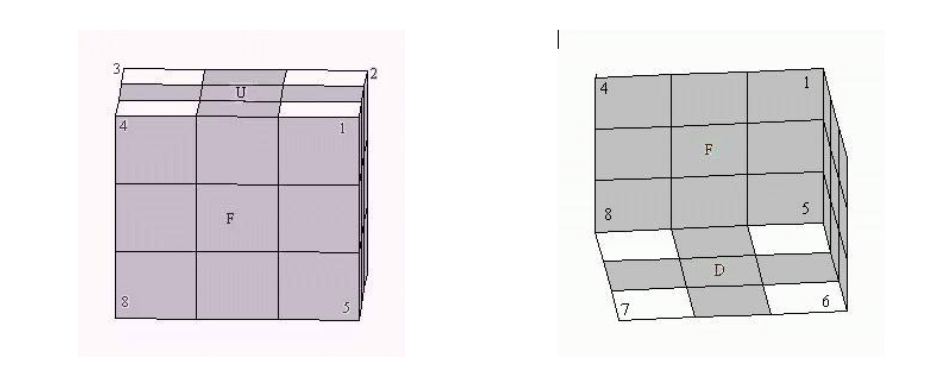
\includegraphics[scale=0.1]{figures/num_coins.png}
    \caption{Numérotation des coins}
    \label{num_coins}
  \end{figure}

  \begin{figure}
    \centering
    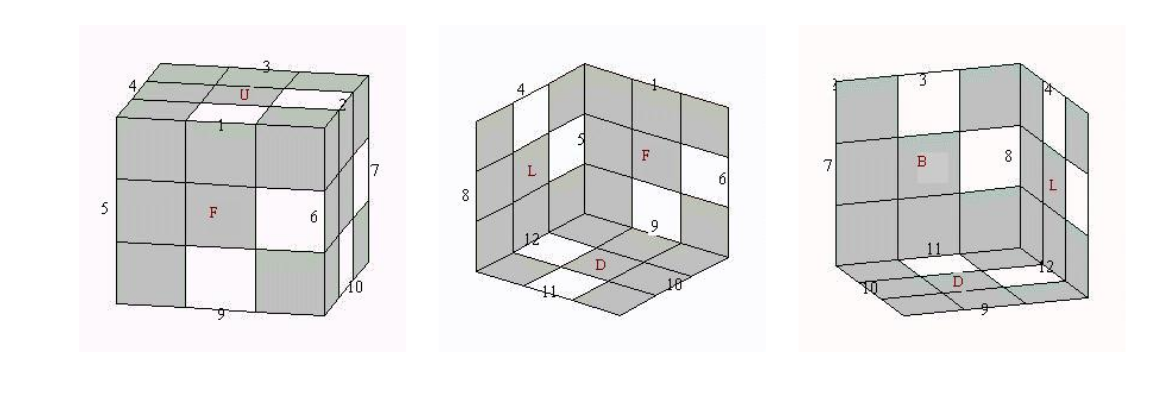
\includegraphics[scale=0.1]{figures/num_aretes.png}
    \caption{Numérotation des arêtes}
    \label{num_aretes}
  \end{figure}
\end{frame}


%--- Next Frame ---%

\begin{frame}
  \frametitle{Groupe du Rubik's cube}
  \begin{enumerate}
    \item $(Rub, \circ)$ contient toutes les transformations du Rubik's cube engendrées par les rotations des 6 tranches.
    \item $Rub$ = groupe de Rubik's cube \emph{légal}, $G \supset Rub$ = groupe du Rubik's cube \emph{illégal} ou élargi.
  \end{enumerate}
\end{frame}

\begin{frame}
  \frametitle{Groupe du Rubik's cube}
  \begin{enumerate}
    \item Posons $G_C$ le groupe d'action sur les coins et $G_A$ le groupe d'action sur les arêtes.
    $G \simeq G_C \times G_A$.
    \item $ord( G_C ) = 8! \times 3 ^{8}$.
    \item $ord( G_A ) = 12! \times 2 ^{12}$.
    \item $ord( G ) = ord( G_C ) \times ord( G_A ) =8! \times 3 ^{8} \times 12! \times 2 ^{12}$.
  \end{enumerate}

  \begin{theorem}
    $Rub$ est un sous-groupe de $G$ d'indice 12.
  \end{theorem}

  \begin{corollary}
    $\mid Rub \mid = \frac{1}{12} \times 8! \times 3 ^{8} \times 12! \times 2 ^{12} \simeq 43 \times 10 ^{18}$.
  \end{corollary}
\end{frame}

\begin{frame}
  \frametitle{Construction du groupe de Rubik's cube}
  Objectif : montrer que $G \simeq ((\mathbb{Z}/{ 3 }\mathbb{Z}) ^{8} \rtimes \mathfrak{S}_{8} ) \times ((\mathbb{Z}/{ 2 }\mathbb{Z}) ^{12} \rtimes \mathfrak{S}_{12} )$.

  \

  $\forall g \in G, g= (\pi_C(g), \pi_A(g))$.

  \begin{enumerate}
    \item $\pi_C : G \to G_C$ est la projection canonique de $G$ sur $G_C$ qui laisse fixe $A$ ;
    \item $\pi_A : G \to G_A$ est la projection canonique de $G$ sur $G_A$ qui laisse fixe $C$.
  \end{enumerate}
\end{frame}

\begin{frame}
  \frametitle{Mélange des coins}
  \begin{figure}
    \centering
    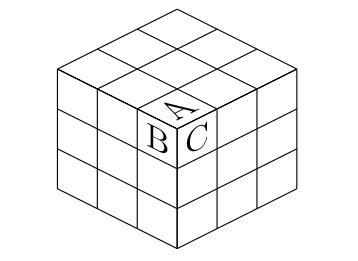
\includegraphics[scale=0.3]{figures/cube_coin.png}
    \caption{Les 3 facettes d'un coin}
    \label{cube_coin}
  \end{figure}
\end{frame}
%--- Next Frame ---%

\begin{frame}
  \frametitle{Mélange des coins}
  \begin{figure}
    \centering
    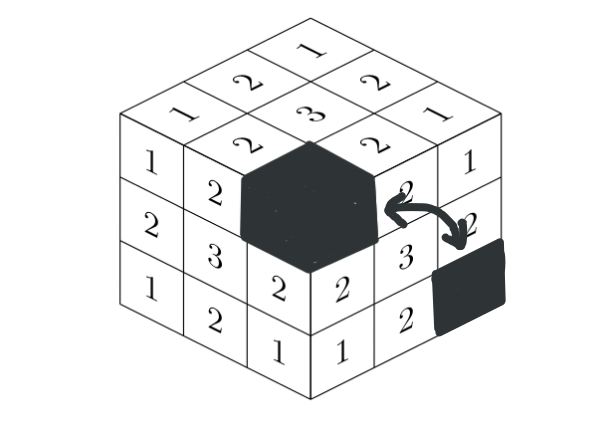
\includegraphics[scale=0.2]{figures/coin-permutations.png}
    \caption{Les permutations des coins}
    \label{coin-permutations}
  \end{figure}

  Si l'on ne regarde que les positions des coins, il existera un morphisme $\sigma_C :
    \begin{array}{ccc}
    G_C & \longrightarrow & \mathfrak{S}_{C} \simeq \mathfrak{S}_{8}   \\
    g & \longmapsto \sigma_C(g)
    \end{array}$.

  \begin{itemize}
    \item $\sigma_C $ surjectif ;
    \item $\operatorname{Ker}(\sigma_C) = Rot_C$, le groupe qui contient les rotations des coins.
  \end{itemize}
\end{frame}
%--- Next Frame ---%

\begin{frame}
  \frametitle{Mélange des coins}

  \begin{itemize}
    \item $\rho_C : G_C \to \mathbb{Z}/{ 3 }\mathbb{Z} ^{8}$ associe à $g \in G_C$ le pivotement des coins.
    \item $\rho_C(g) = (n_1, \dots, n_8)$.
    \item Si $g$ agit sur un coin $j$, alors $g$ orientera le coin $j$ de $n_j$ tiers de tour dans le sens direct.
    \item Groupe cyclique d'ordre 3, donc isomorphe à $\mathbb{Z}/{ 3 }\mathbb{Z}$ ;
    \item $Rot_C \simeq (\mathbb{Z}/{ 3 }\mathbb{Z}) ^{C} \simeq (\mathbb{Z}/{ 3 }\mathbb{Z}) ^{8}$.
  \end{itemize}
\end{frame}
%--- Next Frame ---%

\begin{frame}
  \frametitle{Mélange de coins}
  \begin{table}
    \centering
    \begin{tabular}{|c|c|}
      \hline \\
      $ F$ & $(2,0,0,1,1,0,0,2)$ \\
      \hline \\
      $D$ & $(0,0,0,0,0,0,0,0)$  \\
      \hline \\
      $F \circ U$ & $ (2,0,0,1,1,0,0,2)$ \\
      \hline
    \end{tabular}
    \caption{Les orientations des coins induites par les rotations $F$, $D$, $F \circ U$}
    \label{}
  \end{table}
\end{frame}
%--- Next Frame ---%

\begin{frame}
  \frametitle{Mélange des coins}
  \begin{itemize}
    \item $g \in G_C$ se décompose en le produit $\rho_C(g) \sigma_C(g)$ et cette écriture est unique.
  \end{itemize}

  \begin{remark}
    \begin{equation*}
      hg = \rho_C(h) \sigma_C(h) \rho_C(g) \sigma_C(g) = \underbrace{\rho_C(h) \sigma_C(h) \rho_C(g) \sigma_C(h) ^{-1} }_{\rho_C(hg)} \underbrace{\sigma_C(h) \sigma_C(g)}_{\sigma_C(hg)}.
    \end{equation*}
  \end{remark}

  \begin{itemize}
    \item Relation caractéristique d'un produit semi-direct interne.
    \item $G_C \simeq \mathbb{Z}/{ 3 }\mathbb{Z} ^{8} \rtimes \mathfrak{S}_{8} $.
  \end{itemize}

\end{frame}

%--- Next Frame ---%
\begin{frame}
  \frametitle{Mélange des coins}
  \begin{itemize}
    \item $\forall \rho \in Rot_C, \rho = (n_x) _{x \in C} \in (\mathbb{Z}/{ 3 }\mathbb{Z}) ^{C}$, où chaque coin $x$ subit une rotation de $n_x$ tiers de tour.
    \item Rotation totale de $g$ : $rt_C(g) := \sum_{x \in C} n_x \in \mathbb{Z}/{ 3 }\mathbb{Z} $.
  \end{itemize}

  \begin{lemma}
    $rt_C : (G_C, \circ) \to (\mathbb{Z}/{ 3 }\mathbb{Z}, +)$ est un morphisme de groupes.
  \end{lemma}
\end{frame}
%--- Next Frame ---%

\begin{frame}
  \frametitle{Mélange des coins}

  \begin{remark}
    Pour tout $g, h \in G_C$ tels que $\rho_C(g) = (n_x) _{x \in C}$ et $\rho_C(h) = (n_x') _{ x \in C}$, si l'on note $\rho_C(gh) = (n_x'') _{x \in C}$ on a, pour tout $x \in C$ :

    $$ n_x'' = n_x + n' _{ \sigma ^{-1}(g)(x)}.$$
  \end{remark}

  \begin{figure}[h!]
    \centering
    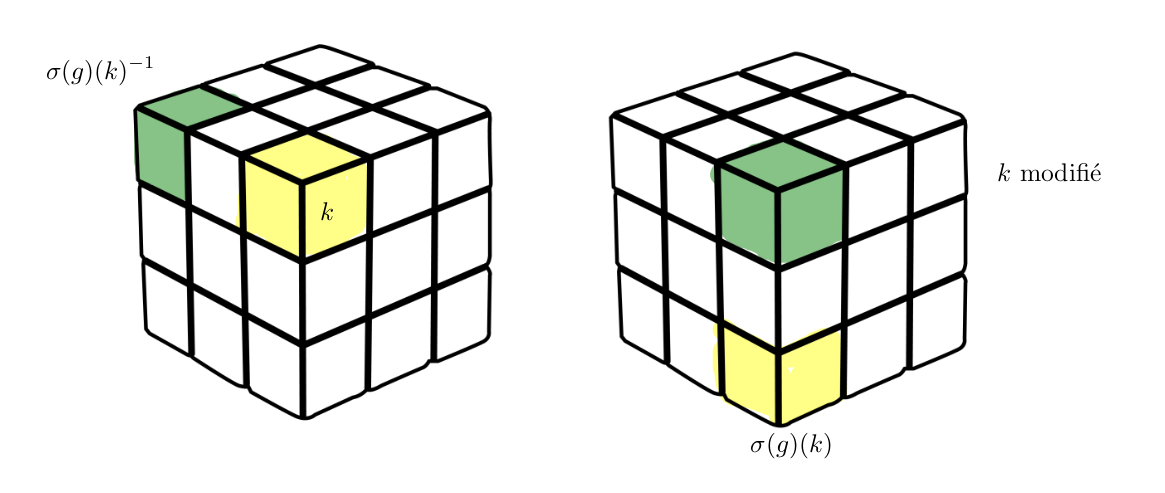
\includegraphics[scale=0.2]{figures/composition_orientations_coins.png}
    \caption{Schéma explicatif}
    \label{}
  \end{figure}
\end{frame}
%--- Next Frame ---%

\begin{frame}
  \frametitle{Mélange des coins}

  \begin{proof}[Démonstration du lemme]
    \begin{itemize}
      \item Soient $g, h \in G_C$, où $g = \rho_C(g) \sigma_C(g) $ et $h = \rho_C(h)\sigma_C(h)$. Notons $gh = \rho_C(gh) \sigma_C(gh)$.
      \item \begin{gather*}
        gh = \rho_C(g) \sigma_C(g) \rho_C(h) \sigma_C(h)\\
         = \underbrace{\rho_C(g) \sigma_C(g) \rho_C(h) \sigma_C(g) ^{-1} }_{\rho_C(gh)} \underbrace{\sigma_C(g) \sigma_C(h)}_{\sigma_C(gh)}.
      \end{gather*}
      \item $\rho_C(gh) = (n_x'') _{x \in C} = n_x + n' _{\sigma_C(g)(x) ^{-1} }$.
      \item $rt_C(gh) = \sum_{x \in C}^{} (n_x + n'_{\sigma_C(g)(x) ^{-1} }) = \sum_{x \in C}(n_x+ n_x').$
    \end{itemize}
  \end{proof}
\end{frame}
%--- Next Frame ---%

\begin{frame}
  \frametitle{Mélange des arêtes}
  \begin{figure}
    \centering
    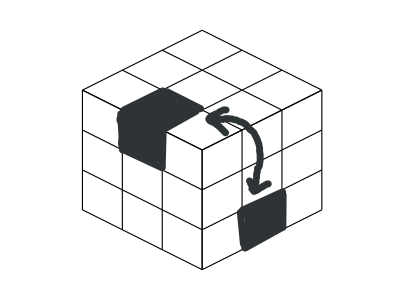
\includegraphics[scale=0.2]{figures/arete-permutation.png}
    \caption{Les permutations des arêtes}
    \label{arete-permutation}
  \end{figure}


    Si l'on ne regarde que les positions des arêtes, il existera un morphisme $\sigma_A :
      \begin{array}{ccc}
      G_A & \longrightarrow & \mathfrak{S}_{A} \simeq \mathfrak{S}_{12}   \\
      g & \longmapsto \sigma_A(g)
      \end{array}$.

    \begin{itemize}
      \item $\sigma_A $ surjectif ;
      \item $\operatorname{Ker}(\sigma_A) = Rot_A$, le groupe qui contient les rotations des arêtes.
    \end{itemize}
\end{frame}

\begin{frame}
  \frametitle{Mélange des arêtes}

  \begin{itemize}
    \item $\rho_A : G_A \to \mathbb{Z}/{ 2 }\mathbb{Z} ^{12}$ associe à $g \in G_A$ le pivotement des arêtes.
    \item $\rho_A(g) = (m_1, \dots, m _{12})$.
    \item Si $g$ agit sur la $j ^{e}$ arête, alors $g$ orientera cette arête de $m_j$ demies de tour.
    \item Groupe cyclique d'ordre 2, donc isomorphe à $\mathbb{Z}/{ 2 }\mathbb{Z}$ ;
    \item $Rot_A \simeq (\mathbb{Z}/{ 2 }\mathbb{Z}) ^{A} \simeq (\mathbb{Z}/{ 2}\mathbb{Z}) ^{12}$.
  \end{itemize}
\end{frame}

\begin{frame}
  \frametitle{Mélange des arêtes}
  \begin{table}[h!]
    \centering
    \begin{tabular}{|c|c|}
      \hline \\
      $F$ & $(1,0,0,0,0,0,0,0,1,0,0,0)$ \\
      \hline \\
      $D$ & $(0,0,0,0,0,0,0,0,0,1,0,1)$ \\
      \hline \\
      $F \circ U$ & $(1,0,1,0,1,0,0,0,1,0,0,0)$ \\
      \hline
    \end{tabular}

    \caption{Les pivotements d'arêtes induites par les mouvements élementaires}
    \label{tableau_orientations_aretes}

  \end{table}

\end{frame}
%--- Next Frame ---%

\begin{frame}
  \frametitle{Mélange des arêtes}
  \begin{itemize}
    \item $g \in G_A$ se décompose en le produit $\rho_A(g) \sigma_A(g)$ et cette écriture est unique.
    \item $G \simeq Rot_A \rtimes \mathfrak{S}_{A} $.
    \item $\forall \rho \in Rot_A, \rho = (m_y) _{y \in A} \in (\mathbb{Z}/{ 2 }\mathbb{Z}) ^{A}$, où chaque arête $y$ subit une rotation de $ m_y$ demis de tour.
    \item Rotation totale de $g$ : $rt_A(g) := \sum_{y \in A} m_y \in \mathbb{Z}/{ 2 }\mathbb{Z} $.
  \end{itemize}

  \begin{lemma}
    $rt_A : (G_A, \circ) \to (\mathbb{Z}/{ 2 }\mathbb{Z}, +)$ est un morphisme de groupes.
  \end{lemma}
\end{frame}

%--- Next Frame ---%

\begin{frame}
  \frametitle{Théorème fondamental du Rubik's cube}
  Soit $g \in G$. On écrit $g = \rho_C \sigma_C \rho_A \sigma_A, \rho_C \in Rot_C, \rho_A \in Rot_A, \sigma_C \in \mathfrak{S}_{C}, \sigma_A \in \mathfrak{S}_{A}$.

  Soit $E : g \to \{ \pm 1 \} $, $E(g) = \varepsilon (\sigma_A(g)) \varepsilon (\sigma_C(g))$.

  On a le morphisme suivant \begin{equation*}
  rt :
   \begin{array}{lll}
   G & \longrightarrow & \{ \pm 1 \} \times (\mathbb{Z}/{ 3 }\mathbb{Z}) \times (\mathbb{Z}/{ 2 }\mathbb{Z}) \\
   g & \longmapsto (E (g), rt_C \circ \pi_C(g), rt_A \circ \pi_A(g))
   \end{array}.
  \end{equation*}

  $[G : \operatorname{Ker}(rt)] = 12$.

  \begin{theorem}
    $Rub=\operatorname{Ker}(rt)$, ie

    $$ g \in G \iff \left \lbrace \begin{matrix}
    E (g)=1 \\
    \sum_{x \in C} n_x = 0 \ [3] \\
    \sum_{y \in A} m_y = 0 \ [2]
    \end{matrix} \right.$$
  \end{theorem}
\end{frame}
%--- Next Frame ---%

\begin{frame}
  Montrons l'inclusion $Rub \subset \operatorname{Ker}(rt)$.

  \begin{itemize}
    \item Un mouvement élementaire induit un 4-cycle sur les coins et un 4-cycle sur les arêtes. Ce sont des cycles à support disjoint. Donc $E(g) =1$ pour tout $g $ produit de mouvements élementaires.
    \item $F$ = ensemble des facettes des arêtes. on a $\mid F \mid = 24$. Un mouvement élementaire induit deux 4-cycles sur les facettes des arêtes. Comme c'est un produit de 4-cycles, il est de signature paire.
    \item On prend deux faces privilégiées $U$ et $D$ par exemple. La rotation $U$ (ou $D$) ne pivote pas les coins. La rotation $F$ (par exemple) pivote les deux coins $x _{U,F,R}$ et $x _{U,F,L}$ de 1 et de 2 tiers de tour. Leur somme est nulle dans $\mathbb{Z}/{ 3 }\mathbb{Z}$.
  \end{itemize}
\end{frame}
%--- Next Frame ---%

\begin{frame}
  \frametitle{Quelques rappels}
  \begin{itemize}
    \item Le groupe $G$ des mouvements du Rubik's cube (y compris illégaux) est isomorphe à $$ ((\mathbb{Z}/{ 3 }\mathbb{Z}) ^{8} \rtimes \mathfrak{S}_{8} ) \times ((\mathbb{Z}/{ 2 }\mathbb{Z}) ^{12} \rtimes \mathfrak{S}_{12} ).$$
    \item Un élément $g \in G$ se décompose naturellement en $g = \sigma_A(g) \rho_A(g) \sigma_C(g) \rho_A(g)$.
  \end{itemize}
On a le morphisme suivant
  \begin{equation*}
 rt :
  \begin{array}{lll}
  G & \longrightarrow & \{ \pm 1 \} \times (\mathbb{Z}/{ 3 }\mathbb{Z}) \times (\mathbb{Z}/{ 2 }\mathbb{Z}) \\
  g & \longmapsto (E (g), rt_C \circ \pi_C(g), rt_A \circ \pi_A(g))
  \end{array}.
 \end{equation*}

  Le sous-groupe $Rub$ de $G$ contient toutes les opérations ``légales''.

\end{frame}
%--- Next Frame ---%

\begin{frame}
  Si $g$ est un mouvement légal, alors $g$ vérifie le théorème suivant :

   \begin{theorem}

     $$ g \in Rub \iff \left \lbrace \begin{matrix}
     E (g) = \varepsilon (\sigma_A(g)) \varepsilon (\sigma_C(g))=1 \\
     \sum_{x \in C} n_x = 0 \ [3] \\
     \sum_{y \in A} m_y = 0 \ [2]
     \end{matrix} \right.$$
   \end{theorem}

   On a montré que $Rub \subset \operatorname{Ker}(rt)$.

   Aujourd'hui, on montrera que $\operatorname{Ker}(rt) \subset Rub$. On présentera aussi quelques sous-groupes du groupe $Rub$, à savoir
   \begin{enumerate}
     \item Le groupe des quaternions ;
     \item Le groupe ``carré'' (square group).
   \end{enumerate}
\end{frame}
%--- Next Frame ---%

\begin{frame}
  \frametitle{Algorithme de résolution du Rubik's cube}
  La démonstration de $\operatorname{Ker}(rt) \subset Rub$ est plutôt constructive. On doit introduire l'algorithme de résolution du Rubik's cube.

  Cet algorithme consiste à :

  \begin{itemize}
    \item mettre les arêtes à leur place ;
    \item les retourner 2 à 2 afin de les orienter correctement ;
    \item appliquer les 2 étapes précédentes aux coins sans toucher aux arêtes.
  \end{itemize}


\textbf{Notations}
\begin{itemize}
  \item $y _{\alpha, \beta }$ l'arête commune aux faces $\alpha, \beta $ ;
  \item $x _{\alpha, \beta, \gamma }$ le coin commun aux faces $\alpha, \beta , \gamma $.
\end{itemize}

On notera $g = \sigma_C(g) \rho_C(g) \sigma_A(g) \rho_A(g) = \sigma_C \rho_C \sigma_A \rho_A$, $\sigma_C \in \mathfrak{S}_{8}, \sigma_A \in \mathfrak{S}_{12}, \rho_C \in \mathbb{Z}/{ 8 }\mathbb{Z} ^{8}, \rho_A \in \mathbb{Z}/{ 2 }\mathbb{Z} ^{12}$.

\end{frame}
%--- Next Frame ---%

\begin{frame}
  \frametitle{Pivotement (rotation) des arêtes}
Cas spécial :  $\sigma_A =id , \sigma_C = id$, $\rho_C = (0, \dots, 0)$.

  $$ h= LF R ^{-1}  F ^{-1}  L ^{-1}  U ^2 RU RU ^{-1}  R ^2 U ^2 R  $$

  pivote $y _{U,F}$ et $y _{U,R}$.
  \begin{figure}[h!]
    \centering
    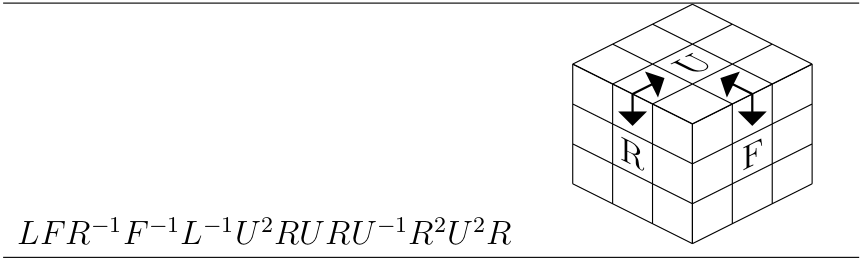
\includegraphics[scale=0.2]{figures/pivote_2_aretes.png}
    \caption{Le mouvement qui pivote deux arêtes}
    \label{pivote_2_aretes}
  \end{figure}


Pour tout couple d'arêtes $(y_1, y_2)$, il existe $g \in Rub$ qui envoie $y_1 $ sur $ y _{U,F}$ et $y_2$ sur $y _{U,R}$. Il s'en suit que $g h g ^{-1} $ réoriente deux arêtes $y_1$ et $y_2$ quelconques.

\end{frame}
%--- Next Frame ---%

\begin{frame}
  \frametitle{Pivotement (rotation) des arêtes}

  \begin{itemize}
    \item $\operatorname{Ker}(\sigma_A \circ \pi_A)$ contient $g \in Rub$ qui laissent invariantes les positions des arêtes, mais qui peuvent éventuellement modifier leur orientation.
    \item $Rot_A ^{0} \subset Rot_A$ = les éléments de rotation totale nulle.
  \end{itemize}

  \begin{lemma}
    $\pi_A : \operatorname{Ker}(\sigma_A \circ \pi_A) \cap Rub \to Rot_A ^{0}$ est surjective.
  \end{lemma}
\end{frame}


%--- Next Frame ---%

\begin{frame}
  \frametitle{Pivotement (rotation) d'arêtes}

  \begin{proof}
    \begin{itemize}
      \item $\forall y_1, y_2 \in A$, il existe $g \in Rub$ tel que $g h g ^{-1} $ retourne $y_1$ et $y_2$ sans toucher aux autres arêtes.
      \item $Rub \cap \operatorname{Ker}(\sigma_A \circ \pi_A)$ contient les rotations d'arêtes légales.
      \item $\pi_A (Rub \cap \operatorname{Ker}(\sigma_A \circ \pi_A))$ contient les retournements d'arêtes quelconques. Les élements de cet ensemble engendrement $Rot_A ^{0}$, car tout $r \in Rot_A ^{0}$ est composé d'un nombre \textbf{pair} de retournements d'arêtes (théorème fondamental).
    \end{itemize}
  \end{proof}
\end{frame}
%--- Next Frame ---%

\begin{frame}
  \frametitle{Pivotement de coins}
  $\sigma_A = id, \sigma_C = id, \rho_A = (0, \dots, 0)$.

  $$ \gamma = (R ^{-1}  D ^2 RB ^{-1} U ^2 B) ^2 $$

  tourne $x _{U,F,R}$ d'un tiers de tour et $x _{B,D,L}$ de deux tiers de tour.

  \begin{figure}[h!]
    \centering
    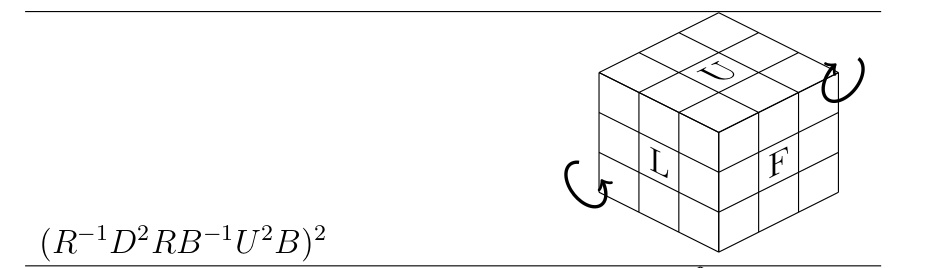
\includegraphics[scale=0.2]{figures/pivote_2_coins.png}
    \caption{Le mouvement pivotant $x _{U,F,R}$ et $x _{B,D,L}$}
    \label{pivote_2_coins}
  \end{figure}

  Pour tout couple $x_1, x_2$ de coins, il existe $g \in Rub$ qui envoie $x_1$ sur $x _{U,F,R}$ et $x_2 $ sur $x _{B,D,L}$. Il s'en suit que $g \gamma g ^{-1} $ réoriente $x_1$ et $x_2$ sans déranger les autres coins.
\end{frame}

%--- Next Frame ---%

\begin{frame}
  \frametitle{Pivotement de coins}

  \begin{itemize}
    \item $Rot_C ^{0} \subset Rot_C$ = les mouvements de rotation totale nulle.
  \end{itemize}

  \begin{lemma}
    $\pi_C : Rub \cap Ker(\sigma_C \circ \pi_C) \to Rot_C ^{0}$ est surjective.
  \end{lemma}

  \begin{proof}
    La démonstration est identique que pour le pivotement des arêtes.
  \end{proof}
\end{frame}
%--- Next Frame ---%

\begin{frame}
  \frametitle{Permutation des arêtes}
  \begin{itemize}
    \item Le mouvement
    \begin{equation}\label{permuter-aretes}
      U ^{-1} F U L U ^{-1} L ^{-1} F ^{-1}
    \end{equation}
    permute deux arêtes de la face $U$.
    \item Par conjugaison de \ref{permuter-aretes}, on peut transposer deux arêtes de $A$.
    \item Les transpositions engendrent $\mathfrak{S}_{A} $. Cela prouve qu'il existe un élement de $Rub$ qui envoie les arêtes à leur emplacements respectifs.
  \end{itemize}


\end{frame}
%--- Next Frame ---%

\begin{frame}
  \frametitle{Permutation des coins}
    \begin{itemize}
      \item Une fois les arêtes mises en place, on sait que la permutation opérant sur les coins doit être paire.
      \item Le groupe alterné $\mathfrak{A}_C$ est engendré par les 3-cycles.
      \item On montre qu'il existe un 3-cycle agissant sur un triplet de coins quelconque.
    \end{itemize}

    \begin{equation*}
      \mu = RB ^{-1}  RF ^2 R ^{-1}  BRF ^2 R ^2
    \end{equation*}

    \begin{figure}[h!]
      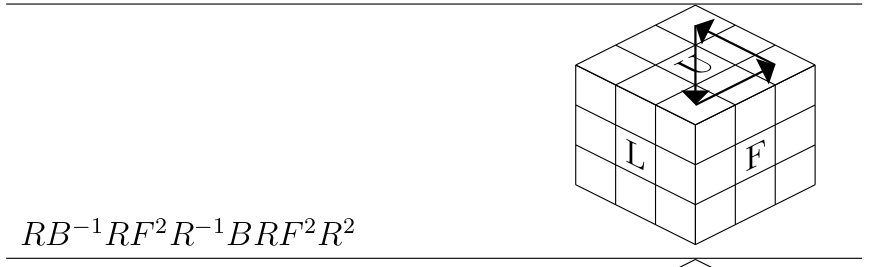
\includegraphics[scale=0.2]{figures/3_cycle_coin.png}
      \caption{Le mouvement $\mu$}
      \label{}
    \end{figure}

    Ce mouvement agit par 3-cycle sur les coins $ x _{U,F,L}, x _{U,F,R}, x _{U,B,R} $ . Pour tout $x \in C$, il existe $g \in Rub$ qui envoie $x$ sur la position d'un de ces 3 coins. On peut ainsi construire un 3-cycle sur n'importe quel triplet de coins.
\end{frame}
%--- Next Frame ---%

\begin{frame}
  \frametitle{Résolution du Rubik's cube}
  \begin{itemize}
    \item $c_0$ est une configuration de $\operatorname{Ker}(rt)$.
    \item On applique à $c_0$ une suite de mouvements $g$ exposés ci-dessus.
    \item On aboutit à $c_0 \circ g = 1 _{Rub}$.
    \item $g ^{-1} = c_0$, donc $c_0 \in Rub$.
    \item Ainsi $\operatorname{Ker}(rt) \subset Rub$. A ce stade, on a prouvé que $\operatorname{Ker}(rt) = Rub$.
  \end{itemize}
\end{frame}
%--- Next Frame ---%

\begin{frame}
  \frametitle{Quelques sous-groupes remarquables du groupe du Rubik's cube}
  \textbf{Le groupe des quaternions}

  Le groupe des quaternions $\mathcal{Q}$ (muni de la multiplication) est défini ainsi :

  $$ \mathcal{Q} = \{ i,j,k \ | \ i ^2 = j ^2 = k ^2 = ijk = -1  \} .$$

\begin{remark}
  \
  \begin{enumerate}
    \item $i,j,k$ sont d'ordre 4 dans $\mathcal{Q}$.
    \item $i ^{-1} = -i$, $j ^{-1} = -j$, $k ^{-1} = -k$.
  \end{enumerate}
\end{remark}
\end{frame}
%--- Next Frame ---%

\begin{frame}
  \frametitle{Le groupe des quaternions}
  On considère les manoeuvres suivantes :
  \begin{enumerate}
    \item $1 : = id$ ;
    \item $-1: = m _{435}$ qui pivote les arêtes $y _{UF}$, $y _{UL}$, $y _{UB}$, $y _{UR}$ d'une demie de tour dans le sens des aiguilles d'une montre ;
    \item $i = m _{706}$ qui transpose $y _{UR}$ et $y _{UF}$ en pivotant $y _{UR}$ d'une demie de tour et qui transpose $y _{UL}$ et $y _{UB}$ en pivotant $ y _{UL}$ d'une demie de tour ;
    \item $j = m _{707}$ qui transpose $y _{UL}$ et $y _{UF}$ en pivotant $y _{UL}$ d'une demie de tour et qui transpose $y _{UB}$ et $ y _{UR}$ en pivotant $ y _{UB}$ d'une demie de tour ;
    \item $k = m _{710}$ qui transpose $y _{UF}$ et $y _{UB}$ en pivotant $y _{UF}$ d'une demie de tour et qui transpose $y _{UL}$ et $y _{UR}$ en pivotant $ y _{UL}$ d'une demie de tour.
  \end{enumerate}

  \begin{figure}[h!]
    \centering
    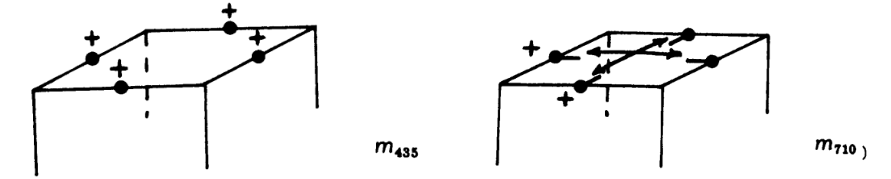
\includegraphics[scale=0.2]{figures/manip_quaternions.png}
    \caption{Les mouvements $m _{435}$ et $m _{710}$}
    \label{}
  \end{figure}
\end{frame}
%--- Next Frame ---%

\begin{frame}
  \frametitle{Le groupe des quaternions}

  On note $\mathcal{R}$ le groupe engendré par $-1 = m _{435}, i = m _{706}, j= m _{707}, k= m _{710}$. On a que $(\mathcal{R}, \circ)$ est un groupe dont les éléments vérifient les propriétés suivantes :

  \begin{gather}
    i ^2 = j ^2 = k ^2 = ijk = -1, \label{quaternions}\\
    ij = -ji = k, jk = -kj = i, ki = -ik = j. \label{quaternions2}
  \end{gather}
  On a un isomorphisme de groupes $\varphi : \mathcal{R} \to \mathcal{Q}$.

  \begin{proof}
  On peut vérifier par un calcul fastidieux que les éléments de $\mathcal{R}$ vérifient les propriétés du groupe de quaternions.
  \end{proof}
\end{frame}

%--- Next Frame ---%

\begin{frame}
  \frametitle{Propriétés du groupe des quaternions}
  Montrons que $\mathcal{Q}$ est d'ordre 8 dont les sous-groupes sont cycliques et distingués dans $\mathcal{Q}$.

  \begin{enumerate}
    \item   $\mathcal{Q} = \{ 1, -1, i,-i,j,-j,k,-k \} $, donc $\mid \mathcal{Q} \mid = 8$.
    \item $\mathcal{Q}$ non commutatif, car $ij = -ji$. Le centre $Z(\mathcal{Q})$ vaut $\{ 1, -1 \} $.
    \item Les sous-groupes de $\mathcal{Q}$ différents de $\{ 1 \} $ et de $\mathcal{Q}$ sont d'ordre 2 ou 4 par le théorème de Lagrange.
    \begin{enumerate}
      \item $\langle -1  \rangle $ est le seul sous-groupe d'ordre 2. S'il existait un sous-groupe d'ordre 2 contenant $i$ (ou $j$, ou $k$), alors il contiendrait aussi 1 et $-i$, donc 3 éléments (c'est absurde).
      \item Les seuls sous-groupes d'ordre 4 sont $\langle i \rangle, \langle j \rangle, \langle k \rangle$. S'il existait un sous-groupe d'ordre 4 contenant $i$ et $j$ par exemple, alors il contiendrait aussi $-i$ et $-j$ ainsi que 1, donc 5 éléments (absurde).
    \end{enumerate}
    Donc tous les sous-groupes de $\mathcal{Q}$ sont cycliques.
  \end{enumerate}

\end{frame}
%--- Next Frame ---%

\begin{frame}
  \frametitle{Propriétés du groupe des quaternions}
  \footnotesize
  \begin{prop}
    Tous les sous-groupes de $\mathcal{Q}$ sont distingués dans $\mathcal{Q}$.
  \end{prop}

  \begin{proof}
  \begin{enumerate}
    \item Le centre $Z(\mathcal{Q}) $, $ \langle -1 \rangle  $, est distingué dans $\mathcal{Q}$ (abélien).
    \item Montrons que $\langle i \rangle $ est distingué. On a

    \begin{gather*}
      j i j ^{-1}  = j i (-j) = -jij = ijj = i (-1) = -i , \\
      k i k ^{-1} = k i (-k) = k(-ik) = kki=-i.
    \end{gather*}

    Donc $\langle i \rangle $ est stable par conjugaison, donc distingué.
  \end{enumerate}
  \end{proof}

  \begin{remark} On peut définir $\mathcal{Q}$ avec des matrices $2 \times 2$ à coefficients dans $\mathbb{C}$
    \begin{gather*}
      1 = \begin{pmatrix}
      1 & 0 \\
      0 & 1
    \end{pmatrix}, I = \begin{pmatrix}
      0 & 1 \\
      -1 & 0
    \end{pmatrix}, J = \begin{pmatrix}
      0 & i \\
      i & 0
    \end{pmatrix}, K = \begin{pmatrix}
      i & 0 \\
      0 & -i
    \end{pmatrix},
    \end{gather*}
  \end{remark}
\end{frame}
%--- Next Frame ---%

\begin{frame}
  \frametitle{Le groupe carré (\emph{square group})}

  On pose $S = \langle U ^2,  F ^2, L ^2, R ^2, D ^2, B ^2 \rangle $.

  \begin{theorem}
    Le groupe carré $S$ est d'ordre $2 ^{13} 3 ^{4}$.
  \end{theorem}

  \begin{proof}
  $S$ agit sur les arêtes et les coins indépendamment.

  On note $\varphi_A$ l'action du groupe $S$ sur l'ensemble des arêtes. Elle admet trois orbites :

  \begin{gather}
    \operatorname{Orb}(y _{UF}) = \{ y _{UF}, y _{UB}, y _{DB}, y _{DF} \} \label{orbite_arete_1}\\
    \operatorname{Orb}(y _{UL}) = \{ y _{UL}, y _{UR}, y _{DR}, y _{DL} \} \label{orbite_arete_2}\\
    \operatorname{Orb}(y _{FL}) = \{ y _{FL}, y _{FR}, y _{BR}, y _{BL} \} \label{orbite_arete_3}
  \end{gather}

  On fait la démonstration pour l'orbite \ref{orbite_arete_1}

  \end{proof}
\end{frame}
%--- Next Frame ---%

\begin{frame}
  \frametitle{Le groupe carré}

  \begin{proof}
    \begin{enumerate}
      \item Montrons que $y _{UF}, y _{UB}, y _{DB}, y _{DF} $ sont bien dans $Orb(y _{UF})$. On applique les mouvements suivants :

      \begin{gather*}
        y _{UF}  \stackrel{U ^2}{\longrightarrow} y _{UB} \\
        y _{UF}  \stackrel{F ^2}{\longrightarrow} y _{DF} \\
        y _{UF}  \stackrel{U ^2 B ^2}{\longrightarrow} y _{DB}.
      \end{gather*}

      \item Montrons qu'aucune autre arête n'est dans $Orb( y _{UF})$. En effet,
      \begin{enumerate}
        \item Le mouvement $U ^2$ échange l'arête $y _{UF}$ et $y _{UB}$ ;
        \item Le mouvement $F ^2$ échange $y _{UF}$ et $y _{DF}$ ;
        \item Le mouvement $B ^2$ échange $ y _{UB}$ et $y _{DB}$ ;
        \item Le mouvement $D ^2$ échange $y _{DF}$ et $y _{DB}$ ;
        \item Les mouvements $L ^2$ et $R ^2$ laissent les 4 arêtes de cette orbite en place.
      \end{enumerate}

    \end{enumerate}
  \end{proof}
\end{frame}
%--- Next Frame ---%

\begin{frame}
  \frametitle{Le groupe carré}

  On note $\varphi_C$ l'action de $S$ sur les coins. Alors

  \begin{gather}
    \operatorname{Orb}(x _{UFL}) = \{ x _{UFL}, x _{UBR}, x _{DFR}, x _{DBL} \} \label{orbite_coins_1} \\
    \operatorname{Orb}(x _{UFR}) = \{ x _{UFR}, x _{ULB}, x _{DRB}, x _{DLF} \} \label{orbite_coins_2} .
  \end{gather}

  \begin{itemize}
    \item On peut placer les arêtes de $(4!) ^{3}$ façons.
    \item $s \in S$ induit une transposition sur une paire d'arêtes d'une orbite donnée.
    \item Condition 1 du théorème fondamental $\implies$ la permutation des coins ainsi que la permutation des arêtes doit être paire. Il reste donc $\frac{(4!) ^{3}}{2} = 2 ^{8} 3 ^{3}$ emplacements possibles pour les arêtes.
    \item Par le théorème fondamental, la rotation totale des coins doit être nulle. Une fois que l'on a placé 4 coins, il reste 4 positions seulement pour les coins restants.
  \end{itemize}
  $$\mid S \mid = \frac{(4!)^{3}}{2} \cdot 4! 4 = 2 ^{8} \cdot 3 ^{3} \cdot 2 ^{5} \cdot 3 = 2 ^{13} \cdot 3 ^{4}.$$
\end{frame}
%--- Next Frame ---%

\begin{frame}
  \begin{figure}
    \centering
    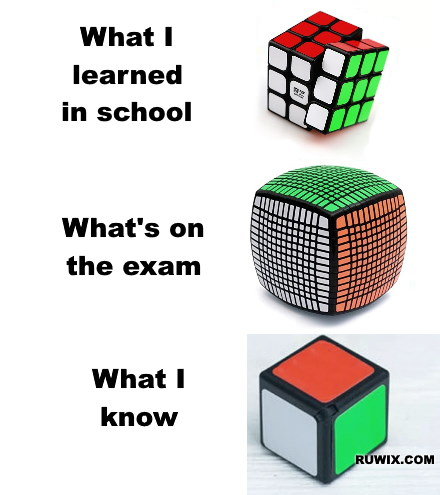
\includegraphics[scale=0.5]{figures/class-vs-exam.jpg}
    \caption{}
    \label{}
  \end{figure}
\end{frame}
%--- Next Frame ---%

\begin{frame}

\end{frame}
%--- Next Frame ---%

\end{document}
